\section{Methods}
\label{sec:methods}

In this manuscript, we are primarily concerned with $k$-NN search in a finite-dimensional space.
Given a dataset $\textbf{X} = \{x_1 \dots x_n\}$, we define a \emph{point} or \emph{datum} $x_i \in \textbf{X}$ as a singular observation, for example, the genome of an organism, the neural-network embedding of an image, etc.

We define a \emph{distance function} $f : \textbf{X} \times \textbf{X} \mapsto \mathbb{R}^+ \ \cup \ \{0\}$ which, given two points $x, y \in \textbf{X}$, deterministically returns a non-negative real number.
% Najib: I don't like the ``have an identity'' wording here. The Measure Theory A-Grader will have to prove her chops for this one.
We require that the distance function be symmetric (i.e., $f(x, y) = f(y, x) \ \forall \ x, y \in \textbf{X}$) and have an identity (i.e. $f(x, y) = 0 \iff x = y$).
If, in addition to these constraints, the distance function obeys the triangle inequality (i.e. $f(x, y) \leq f(x, z) + f(z, y) \ \forall \ x, y, z \in \textbf{X}$), then the distance function is also a \emph{distance metric}.
For example, Euclidean, Levenshtein and Dynamic Time Warping (DTW)~\cite{muller2007dynamic} distances are all distance metrics while Cosine distance is not a metric because it does not obey the triangle inequality.
Under distance metrics, all search algorithms in CAKES are exact.

The choice of distance function varies by dataset.
For example, with neural-network embeddings, one could use Euclidean (L2) or Cosine distance.
With genomic or proteomic data, Levenshtein or Hamming distances are more appropriate.
With time-series data, one could use Dynamic Time Warping (DTW) distance.

% Najib: Reword the following sentence.
CAKES assumes the manifold hypothesis~\cite{fefferman2016testing}, i.e., high-dimensional data collected from constrained generating phenomena typically only occupy a low-dimensional manifold within their embedding space, and exploits this low \emph{local fractal dimension} (LFD) to improve the performance of its search.
We define LFD at some length scale around a point in the dataset as:

\begin{equation}
    \frac{\text{log} \left( \frac{|B_X(q, r_1)|}{|B_X(q, r_2)|} \right) }{\text{log} \left( \frac{r_1}{r_2} \right) }
    \label{eq:methods:lfd-original}
\end{equation}

where $B_X(q, r)$ is the set of points contained in the metric ball of radius $r$ centered at a point $q$ in the dataset $\textbf{X}$.
We stress that this concept differs from the \emph{embedding dimension} of a dataset.
To illustrate the difference, consider SDSS's APOGEE dataset, wherein each datum is a nonnegative real-valued vector of length 8,575.
Hence, the \emph{embedding dimension} of this dataset is 8,575. 
However, due to physical constraints (namely, the laws of physics that govern stellar fusion and spectral emission lines), the data are constrained to a lower-dimensional manifold within the 8,575-dimensional embedding space.
LFD is an approximation of the dimensionality of that lower-dimensional manifold in the ``vicinity'' of a given point.
Figure~\ref{fig:results:lfd-plots} illustrates this concept, showing how real datasets obey the manifold hypothesis.


\subsection{Clustering}
\label{subsec:methods:clustering}

We define a \emph{cluster} as a set of points with a \emph{center} and a \emph{radius}.
The \emph{center} is the geometric median of the points (or a smaller sample of the points) in the \emph{cluster}, and so it is a real data point.
The \emph{radius} is the maximum distance from the \emph{center} to any point in the \emph{cluster}.
Each non-leaf cluster has two child clusters in much the same way that a node in a binary tree has two child nodes.
Hereafter, when we refer to LFD, it is estimated at the scale of the cluster radius and half that radius. 
This allows us to rewrite Definition~\ref{eq:methods:lfd-original} as:

\begin{equation} 
    \log_2 \left( \frac{|B_X(q, r)|}{|B_X(q, r/2)|} \right)
    \label{eq:methods:lfd-simplified}
\end{equation}

In~\cite{yu2015entropy}, metric entropy for a given cluster radius $r$ was defined as the number of clusters of a uniform radius $r$ needed to cover all data.
In this paper, we define the metric entropy $\mathcal{N}_{\hat{r}}(X)$ of a dataset $X$ for the hierarchical clustering scheme as the number of leaf clusters in the tree.

We start by performing a divisive hierarchical clustering on the dataset using CLAM.
The procedure is similar to that outlined in CHESS, but with the following improvements:
better selection of poles for partitioning (see Algorithm~\ref{alg:methods:clustering:partition}) and depth-first reordering of the dataset (see Section~\ref{subsubsec:methods:clustering:dataset-depth-first-reordering}). 

CAKES assumes the manifold hypothesis. 
In other words, we assume that the dataset is embedded in a $D$-dimensional space, but that the data only occupy a $d$-dimensional manifold, where $d \ll D$. 
While we sometimes use Euclidean notions, such as voids, volumes and proximity, to talk about the geometric and topological properties of clusters and of the manifold, CLAM does not rely on such notions; 
they serve merely as a convenient and intuitive way to discuss the underlying mathematics.


\subsubsection {Cluster Partitioning}
\label{subsubsec:methods:cluster-partitioning}

For a cluster $C$ with $|C|$ points, we begin by taking a random sample of $\sqrt{|C|}$ of its points, and computing pairwise distances between all points in this sample.
Using these distances, we compute the \emph{geometric median} of this sample; in other words, we find the point which minimizes the sum of distances to all other points in the sample.
This geometric median is the \emph{center} of $C$.

The \emph{radius} of $C$ is the maximum distance from the \emph{center} to any other point in $C$.

The point which is responsible for that radius (i.e., the furthest point from the \emph{center}) is designated the \emph{left pole}.
The point which is furthest from \emph{left pole} is designated the \emph{right pole}.

We then partition the cluster into a \emph{left child} and a \emph{right child}, where the left child contains all points in the cluster which are closer to the \emph{left pole} than to the \emph{right pole}, and the right child contains all points in the cluster which are closer to the \emph{right pole} than to the \emph{left pole}.
Without loss of generality, we assign to the left child those points which are equidistant from the two poles.

Starting from a root cluster containing the entire dataset, we repeat this procedure until each leaf contains only one datum, or we meet some other user-specified stopping criteria.
This process is described in Algorithm \ref{alg:methods:clustering:partition}.

During the partitioning process, we also compute (and cache) the LFD of each cluster using Equation~\ref{eq:methods:lfd-simplified}.

\begin{algorithm} % enter the algorithm environment
    \caption{Partition(\emph{C})} % give the algorithm a caption
    \label{alg:methods:clustering:partition} % and a label for \ref{} commands later in the document
    \begin{algorithmic} % enter the algorithmic environment
        \REQUIRE $C$, a cluster
        \STATE $seeds \Leftarrow \lfloor \sqrt{|C|} \rfloor$ random points from $C$
        \STATE $c \Leftarrow$ geometric median of $seeds$
        \STATE $l \Leftarrow \argmax f(c, x) \ \forall \ x \in C$
        \STATE $r \Leftarrow \argmax f(l, x) \ \forall \ x \in C$
        \STATE $L \Leftarrow \{x \ | \ x \in C \land f(l, x) \le f(r, x)\}$
        \STATE $R \Leftarrow \{x \ | \ x \in C \land f(r, x) < f(l, x)\}$
        \IF{$|L| > 1$}
            \STATE Partition($L$)
        \ENDIF
        \IF{$|R| > 1$}
            \STATE Partition($R$)
        \ENDIF
    \end{algorithmic}
\end{algorithm}


\subsubsection {Depth-First Reordering}
\label{subsubsec:methods:clustering:dataset-depth-first-reordering}

CAKES also improves upon CHESS by reordering the dataset in depth-first order of traversal of the tree.

In CHESS, each cluster stored a list of indices into the dataset.
This list was used to retrieve the clusters' points during search.
Though this approach allowed us to retrieve the points in constant time, its memory cost was prohibitively high.
With a dataset of cardinality $n$ and each cluster storing a list of indices for its points, we stored a total of $n$ indices at each depth in the tree.
Assuming a balanced tree, and thus $\mathcal{O}\log(n)$ depth, this approach had a memory overhead of $\mathcal{O}(n\log(n))$.

One may improve this memory overhead to $\mathcal{O}(n)$ by only storing indices at the leaf clusters.
This approach, however, introduces a time cost of $\mathcal{O}(n\log(n))$ whenever we need to find the indices for a non-leaf cluster (because it requires a traversal of the subtree rooted at that cluster).

In this work, we introduce a new approach wherein, after building the cluster tree, we reorder the dataset so that points are stored in a depth-first order.
Then, within each cluster, we need only store its \emph{cardinality} and an \emph{offset} to access the its points from the dataset.

The root cluster has an offset of zero and a cardinality equal to the number of points in the dataset.
A left child has the same offset as that of its parent, and the corresponding right child has an offset equal to the left child's offset plus the left child's cardinality.

With no additional memory cost nor time cost for retrieving points during search, depth-first reordering offers significant improvements over the approach used in CHESS.

% % WE WILL USE THIS FOR COMPRESSION, so removing it for now 

% \subsubsection {Scaling Behavior of Cluster Radii}
% \label{subsubsec:methods:clustering:guaranteed-decrease-in-cluster-radii}

% While it may be tempting to assume that cluster radii decrease with each application of Partition (refer to Algorithm \ref{alg:methods:clustering:partition}), unfortunately, this assumption is incorrect. 
% Fortunately, we \emph{can} make some guarantees about the scaling behavior of cluster radii;
% in particular, we prove in this section that cluster radii will stop increasing after at most $d$ partitions, where $d$ is the fractal dimensionality of the dataset. 

% We can describe a $d$-dimensional distribution of data by choosing some set of $d$ mutually orthogonal axes.
% Let $2R$ be the maximum pairwise distance among the points in the dataset. 
% We choose the axes such that the two points that are $2R$ apart lie \emph{along one of the axes}. 
% Thus, a $d$-dimensional hyper-sphere of radius $R$ would bound the dataset. 
% In the worst case, (i.e., with a uniform-density distribution that fills the $d$-sphere), our axes will be such that $2R$ is the maximum pairwise distance \emph{along every axis}. 
% Such a distribution would also produce a balanced cluster tree.

% In this case, Partition will select a maximally distant pair of points to use as poles;
% without loss of generality, say it chooses two points at the extrema one of the $d$ axes. 
% After one partition, the maximum pairwise distance along that axis will be halved, i.e. bounded above by $R$.
% The next recursive Partition will select another of the $d$ axes, and once again, the distance along that axis will be bounded above by $R$
% Thus, after at most $d$ partitions, the maximum pairwise distance along each axis will be bounded above by $R$. 
% The overall (i.e., not restricted to one axis) maximum pairwise distance 
% will be bounded above by $R\sqrt{2}$ by, for example, two instances that lie at the extrema of different axes. 
% See Figure~\ref{fig:methods:scaling-behavior} for an example.

% Thus, starting with a cluster $C$ of radius $R$, after at most $d$ Partitions, the descendants of $C$ will each have radius
% bounded above by $\frac{R}{\sqrt{2}}$. In other words, cluster radii are guaranteed to decrease by a multiplicative factor of $\frac{\sqrt{2}}{2}$ after at 
% most $d$ partitions. 

% Note that, in practice, we never see a balanced clustering.
% Partition produces unbalanced trees due to the varying density of the sampling in different regions of the manifold and the low dimensional ``shape'' of the manifold.
% Further, in practice, the cluster radii decrease by a factor much larger than $\frac{\sqrt{2}}{2}$ with almost every partition;
% the upper bound of $d$ partitions is seldom realized. 

% \begin{figure}[ht!]
%     \centering
%     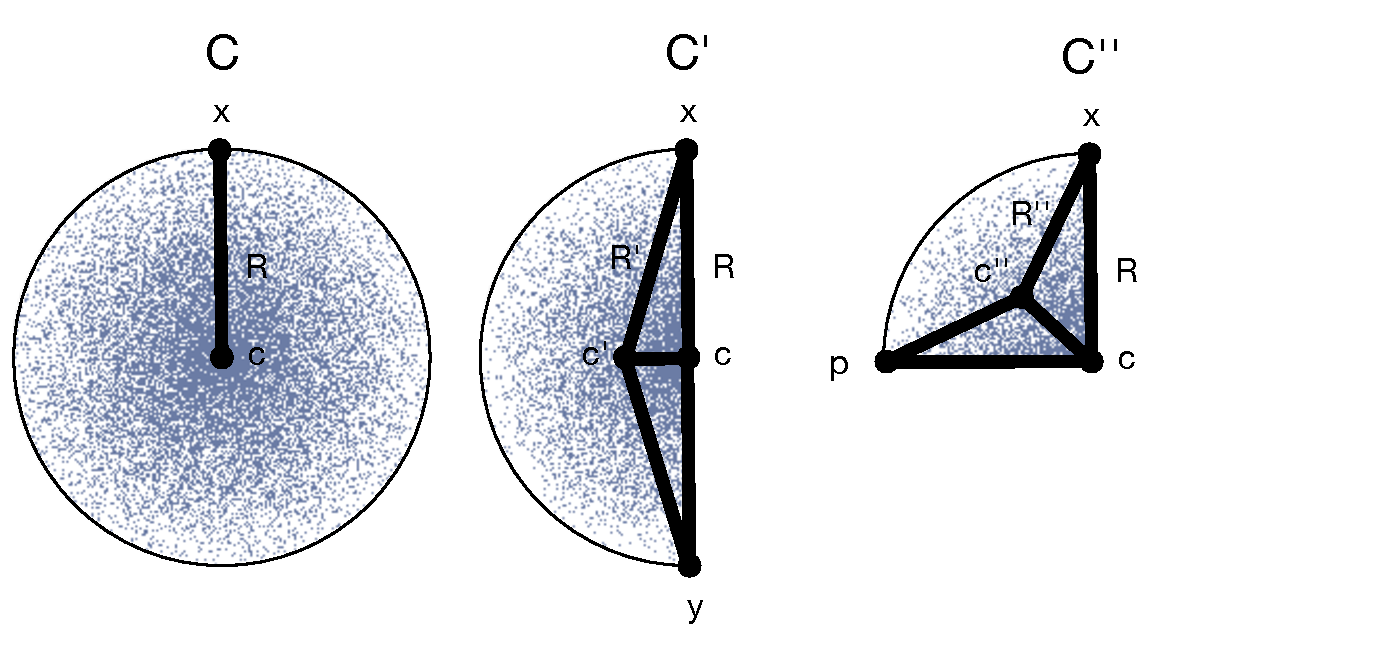
\includegraphics[width=3.4in]{images/geometry/geometry.pdf}
%     \caption{
%         Scaling behavior of radii on a uniform-density disk, which represents the worst-case scenario for a two-dimensional distribution. 
%         $R_0$ denotes the radius of the root cluster $C_0$, and $o_0$ denotes its center. 
%         After one application of Algorithm~\ref{alg:methods:clustering:partition}, we have $C_1$, with radius $R_1$ and center $o_1$.
%         The right triangle formed by $o_0$, $o_1$, and $y_+$ in $C_1$ shows that $R_0 < R_1$.
%         Hence, the radius of a child cluster can be larger than its parent.
%         However, after another application of Algorithm~\ref{alg:methods:clustering:partition}, we have consumed all $d$ orthogonal axes, 
%         as shown in $C_2$.
%         Now, clearly $R_2 < R_0$.
%         In fact, for each subsequent application of Algorithm~\ref{alg:methods:clustering:partition}, the radius of the resulting cluster is bounded above by $\frac{\sqrt{2}R}{2}$.
%     }
%     \label{fig:methods:scaling-behavior}
% \end{figure}


\subsubsection {Complexity}
\label{subsubsec:methods:clustering:clustering:complexity}

The asymptotic complexity of Partition is the same as described in~\cite{ishaq2019clustered}.
By using an approximate partitioning with a $\sqrt{n}$ sample, we achieve $\mathcal{O}(n)$ cost of partitioning and $\mathcal{O}(n \log n)$ cost of building the tree.
This is a significant improvement over exact partitioning and tree-building, which cost $\mathcal{O}(n^2)$ and $\mathcal{O}(n^2 \log n)$ respectively.


\subsection{The Search Problem}
\label{subsec:methods:the-search-problem}

Given Algorithm~\ref{alg:methods:clustering:partition}, we can now pose the $k$-NN and $\rho$-NN search problems.

Given a query $q$, along with a distance function $f$ defined on a dataset $\textbf{X}$, $k$-nearest neighbors search aims to find the set $S_q$ such that $|S_q| = k$ and $\forall x \in \textbf{X} \setminus S_q$, $\ f(x, q) > \max\{f(y, q): y \in S_q \}$;
in other words, for a given $k$, $k$-NN finds the $k$ closest points to $q$ in $\textbf{X}$.
We also have the $\rho$-nearest neighbors search problem, which aims to find the set $\{x \in \textbf{X}: f(q, x) \leq \rho \}$;
that is, find all points in $\textbf{X}$ that are no more than a distance $\rho$ from $q$.

Given a Cluster $C$, let $c$ be its center and $r$ be its radius. Our $\rho$- and $k$-NN algorithms make use of the following properties, as illustrated in Figure~\ref{fig:methods:deltas}.

\begin{itemize}
    \item $\delta = f(q, c)$ is the distance from the query to the cluster center $c$.
    \item $\delta^{+} = \delta + r$ is the distance from the query to the theoretically farthest point in $C$.
    \item $\delta^{-} = \text{max}(0, \delta - r)$ is the distance from the query to the theoretically closest point in $C$.
\end{itemize}

% Najib: For this figure, I want the red, green and blue lines/braces to be thinner. Perhaps 1/2 to 2/3 as thick. Also, I changed the notation for the deltas because it makes things easier in the Sieve and Greedy Sieve algorithms' sections.
\begin{figure}[ht!]
    \centering
    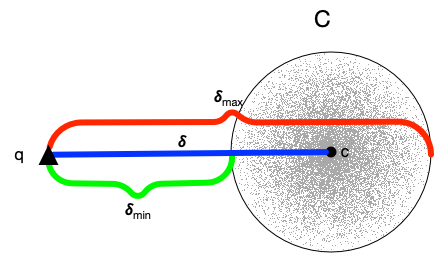
\includegraphics[scale=0.5]{images/geometry/deltas.png}
    \caption{$\delta$, $\delta^{+}$, and $\delta^{-}$ for a cluster $C$ and a query $q$.}
    \label{fig:methods:deltas}
\end{figure}

We define a \emph{singleton} as a cluster which either contains a single point (i.e., has cardinality 1) or which contains duplicates of the same point (i.e., has cardinality greater than 1 but contains only one \emph{unique} point).
A singleton clearly has zero radius, and so $\delta = \delta^{-} = \delta^{+}$.
Hence, we overload the above notation to also refer to the distance from a query to an individual point.


\subsection{\texorpdfstring{$\rho$}{p}-Nearest Neighbors Search}
\label{subsec:methods:rnn-search}

We conduct $\rho$-nearest neighbors search as described in~\cite{ishaq2019clustered}, but with the following improvement:
when a cluster overlaps with the query ball, instead of always proceeding with both of its children, we proceed only with those children which might contain points in the query ball.

% Najib: Visually, ``m'' is not centered on the line segment. It's a little bit to the right. Moving ``l'' to the right is probably the easiest fix.
\begin{figure}[ht!]
    \centering
    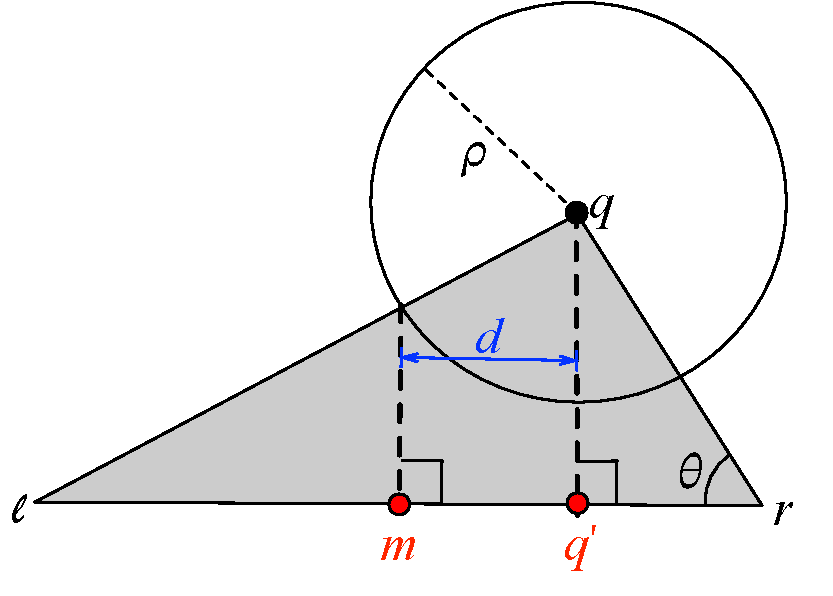
\includegraphics[scale=0.5]{images/geometry/overlapping-children-3.pdf}
    \caption{
        $m$ denotes the midpoint of $\overline{l r}$. $q'$ is the projection of $q$ onto $\overline{l r}$.
        $d$ is the distance from $q'$ to $m$.
        If $d \leq \rho$, both child clusters could contain points in the query ball.
        Otherwise, only the right child cluster could contain such points. 
    }
    \label{fig:methods:overlapping-children-3}
\end{figure}

To determine whether both children can contain points in the query ball, we consider Figure~\ref{fig:methods:overlapping-children-3}.
Here, we overload the notation for $\overline{x y}$ to refer to the line segment joining points $x$ and $y$ as well as the length of that line segment.

Let $q$ denote the query, $\rho$ denote the search radius, and $l$ and $r$ denote the cluster's left and right poles (see Section~\ref{subsubsec:methods:cluster-partitioning}).
Without loss of generality, we assume that $\overline{q r \vphantom{l}} \leq \overline{q l}$ (i.e., the query is closer to $r$ than to $l$).

Now let $q'$ be the projection of $q$ to $\overline{l r}$, $m$ be the midpoint of $\overline{l r}$ and $d$ be the distance from $q'$ to $m$.
Since we assign a point in the parent cluster to the left child if it is closer to the left pole, if $d > \rho$ then the left child cannot contain points inside the query ball.
In this case, we proceed only with the right child.
If, however, $d \leq \rho$ then both child clusters could contain points in the query ball, and so we proceed with both of them.

To check whether $d \leq \rho$, we note that

\begin{equation}
    d = \overline{m q' \vphantom{l}} = \overline{m r \vphantom{l}} - \overline{q' r \vphantom{l}} = \frac{\overline{l r}}{2} - \overline{q' r \vphantom{l}}.
    \label{eq:methods:d-expression}
\end{equation}

Let $\theta$ denote $\angle l r q$, as shown in Figure~\ref{fig:methods:overlapping-children-3}.
By the Law of Cosines on $\triangle l r q$, we have that

\begin{equation}
    \text{cos}(\theta) = \tfrac{\overline{q r \vphantom{l}}^2 + \ \overline{l r}^2 - \ \overline{q l}^2}{2 \cdot \overline{l r} \cdot \overline{q r \vphantom{l}}}.
    \label{eq:methods:cosine-law}
\end{equation}

Since $\triangle r q q'$ is a right triangle, we also have that

\begin{equation}
    \text{cos}(\theta) = \tfrac{\overline{q' r \vphantom{l}}}{\overline{q r \vphantom{l}}}.
    \label{eq:methods:cosine-law-right-triangle}
\end{equation}

Combining Equations~\ref{eq:methods:cosine-law} and~\ref{eq:methods:cosine-law-right-triangle}, we have that

\begin{equation}
    \overline{q' r \vphantom{l}} = \tfrac{\overline{q r \vphantom{l}}^2 + \ \overline{l r}^2 - \ \overline{q l}^2}{2 \cdot \overline{l r}}.
    \label{eq:methods:q-prime-r}
\end{equation}

Substituting Equation~\ref{eq:methods:q-prime-r} into Equation~\ref{eq:methods:d-expression}, we have that

\begin{equation*}
    d = \tfrac{\overline{l r}}{2} - \tfrac{\overline{q r \vphantom{l}}^2 + \ \overline{l r}^2 - \ \overline{q l}^2}{2 \cdot \overline{l r}} = \tfrac{\overline{q l}^2 - \overline{q r \vphantom{l}}^2}{2 \cdot \overline{l r}}.
\end{equation*}

Thus,

\begin{equation}
    d \leq \rho \iff (\overline{q l} + \overline{q r \vphantom{l}})(\overline{q l} - \overline{q r \vphantom{l}}) \leq 2 \cdot \overline{l r} \cdot \rho.
    \label{eq:methods:check-d}
\end{equation}

Note, in particular, that Equation~\ref{eq:methods:check-d} only requires distances between real points, and so it can be used with any distance function, even when $q'$ and $m$ are not real points or cannot be imputed from the data.

To perform $\rho$-nearest neighbors search, we first perform a coarse tree-search, as outlined in Algorithm~\ref{alg:methods:rnn:tree-search}, to find the leaf clusters which overlap with the query ball or any clusters which lie entirely within the query ball.
Then, for all such clusters, we perform a finer-grained search, as outlined in Algorithm~\ref{alg:methods:rnn:leaf-search}, to find all points in which are within a distance $\rho$ of the query.

\begin{algorithm} 
    \caption{tree-search($C$, $q$, $\rho$)} 
    \label{alg:methods:rnn:tree-search} 
    \begin{algorithmic}
        \REQUIRE $C$, a cluster
        \REQUIRE $q$, a query
        \REQUIRE $\rho$, a search radius

        \STATE $c$ $\Leftarrow$ \emph{center} of $C$
        \STATE $r$ $\Leftarrow$ \emph{radius} of $C$

        \IF{$C$ is a leaf \textbf{or} $f(q, c) + r \leq \rho$}
            \STATE \textbf{return} $\{C\}$
        \ELSIF{Inequality~\ref{eq:methods:check-d} is true}
            \STATE $L$ $\Leftarrow$ \emph{left child} of $C$
            \STATE $R$ $\Leftarrow$ \emph{right child} of $C$
            \STATE \textbf{return} tree-search($L, q, \rho$) $\cup$ tree-search($R, q, \rho$)
        \ELSIF{$f(q, l) < f(q, r)$}
            \STATE \textbf{return} tree-search($L, q, \rho$)
        \ELSE
            \STATE \textbf{return} tree-search($R, q, \rho$)
        \ENDIF
    \end{algorithmic}
\end{algorithm}

\begin{algorithm} 
    \caption{leaf-search($S$, $q$, $\rho$)} 
    \label{alg:methods:rnn:leaf-search} 
    \begin{algorithmic}
        \REQUIRE $S$, a set of clusters
        \REQUIRE $q$, a query
        \REQUIRE $\rho$, a search radius

        \STATE $H \Leftarrow \emptyset$, a set of hits

        \FOR{$C \in S$}
            \STATE $c$ $\Leftarrow$ \emph{center} of $C$
            \STATE $r$ $\Leftarrow$ \emph{radius} of $C$
            \IF{$f(q, c) + r \leq \rho$}
                \STATE $H$ $\Leftarrow$ $H \cup \{C\}$
            \ELSE
                \FOR{$p \in C$}
                    \IF{$f(p, q) \leq \rho$}
                        \STATE $H$ $\Leftarrow$ $H \cup \{p\}$
                    \ENDIF
                \ENDFOR
            \ENDIF
        \ENDFOR

        \STATE \textbf{return} $H$
    \end{algorithmic}
\end{algorithm}

\begin{algorithm} 
    \caption{$\rho$-NN-search($root$, $q$, $\rho$)} 
    \label{alg:methods:rnn:rnn-search} 
    \begin{algorithmic}
        \REQUIRE $root$, the root cluster
        \REQUIRE $q$, a query
        \REQUIRE $\rho$, a search radius

        \STATE $S$ $\Leftarrow$ tree-search($root$, $q$, $\rho$)
        \STATE $H$ $\Leftarrow$ leaf-search($S$, $q$, $\rho$)
        \STATE \textbf{return} $H$
    \end{algorithmic}
\end{algorithm}

The asymptotic complexity of $\rho$-nearest neighbors is the same as in~\cite{ishaq2019clustered}, namely:

\begin{gather}
    \mathcal{O}
    \Bigg(
        \underbrace{\log_2 \mathcal{N}_{\hat{r}}(X)}_{\textrm{metric entropy}} +
        \overbrace{ \left| B_X(q, \rho) \right|}^{\textrm{output size}}
        \underbrace{ \left( 1 + \frac{2 \cdot \hat{r}}{ \rho} \right) ^ d}_{\textrm{scaling factor}}
    \Bigg)
    \label{eq:methods:rnn:complexity}
\end{gather}

where $\hat{r}$ is the \textit{mean} radius of leaf clusters, $\mathcal{N}_{\hat{r}}(X)$ is the metric entropy at that radius, $B_X(q, \rho)$ is a ball of radius $\rho$ around the query $q$, and $d$ is the LFD around the query in a region of radius $r$.
From Algorithm~\ref{alg:methods:rnn:rnn-search}, we have that $H = B_X(q, \rho)$, and so $\rho$-nearest neighbors search performance scales linearly with the size of the output set and exponentially with the local fractal dimension around the query.
While one might worry that the exponential scaling factor would dominate, the manifold hypothesis suggests that the local fractal dimension around the query is typically very low, and so this algorithm actually scales sub-linearly with the cardinality of the dataset.


\subsection{\texorpdfstring{$k$}{k}-Nearest Neighbors Search}
\label{subsec:methods:knn-search}

In this section, we present three novel algorithms for exact $k$-nearest neighbors search:
Repeated $\rho$-NN, Sieve, and Greedy Sieve.

In these algorithms, we use $H$, for \emph{hits}, to refer to the data structure which stores the closest points to the query found so far and $Q$ to refer to the data structure which stores the clusters and points which are still in contention for being one of the $k$ nearest neighbors.


\subsubsection{Repeated \texorpdfstring{$\rho$}{p}-NN}
\label{subsubsec:methods:knn-search:repeated-rnn}

In this algorithm, we perform $\rho$-nearest-neighbors search starting with a small search radius, and repeatedly increasing the radius until $|H| \geq k$.

Let the search radius, $r$, be equal to the radius of the root cluster divided by the cardinality of the dataset.
We perform tree-search with radius $r$.
If no clusters are returned, then we double $r$ and perform tree-search again, repeating until we find at least one cluster.
Let $S$ be the set of clusters returned by the first tree-search which returns at least one cluster.

Now, so long as $\sum_{C \in S} |C| < k$, we continue to perform tree-search, but instead of doubling $r$ on each iteration, we multiply it by a factor determined by the LFD in the vicinity of the query ball. 
In particular, we increase the radius by a factor of

\begin{equation}
    \min \left(2, \left( {\frac{k}{\sum_{C \in S} |C|}} \right)^{\mu^{-1}} \right)
    \label{eq:repeated-rnn-factor}
\end{equation}

where $\mu$ is the harmonic mean of the LFD of the clusters in $S$.
We use the harmonic mean to ensure that $\mu$ is not dominated by outlier clusters with very high LFD. 
Intuitively, the factor by which we increase the radius should also be \emph{inversely} related to the number of points found so far. 
Additionally, when the LFD at the radius scale from the previous iteration is low, this suggests that the data are relatively concentrated in that region.
In such a region, a small increase in the radius would likely encounter unoccupied space, so a larger radial increase is needed.
Thus, the factor of radius increase should be \emph{inversely} related to the LFD.

Once $\sum_{C \in S} |C| >= k$, we are guaranteed to have found at least $k$ neighbors, and so we can stop increasing the radius.
We perform $\rho$-nn-search with radius $r$ and return the $k$ nearest neighbors.

\begin{algorithm} % enter the algorithm environment
    \caption{repeated-$\rho$-NN($root$, $q$, $k$)} % give the algorithm a caption
    \label{alg:knn:repeated-rnn} % and a label for \ref{} commands later in the document
    \begin{algorithmic} % enter the algorithmic environment
        \REQUIRE $root$, the root cluster
        \REQUIRE $q$, a query
        \REQUIRE $k$, the number of neighbors to find

        \STATE $r \Leftarrow radius$ of the $root$ cluster
        \STATE $r \Leftarrow$ $\frac{r}{|root|}$
        \STATE $S \Leftarrow \emptyset$, a set of clusters

        \WHILE {$S = \emptyset$}
            \STATE $S \Leftarrow$ tree-search($root$, $q$, $r$)
            \STATE $r \Leftarrow 2 \cdot r$
        \ENDWHILE

        \ALOOP{}
            \IF{$\sum_{C \in S} |C| >= k$}
                \STATE \textbf{break}
            \ENDIF
            \STATE $\mu \Leftarrow \frac{|S|}{\sum_{C \in S} \frac{1}{LFD(C)}}$
            \STATE $r \Leftarrow r \cdot \min \left( 2, \left( {\frac{k}{\sum_{C \in S} |C|}} \right)^{\mu^{-1}} \right)$
            \STATE $S \Leftarrow$ tree-search($root$, $q$, $r$)
        \ENDLOOP

        \STATE $H \Leftarrow$ sort($\rho$-NN-search($root$, $q$, $r$))
        \STATE \textbf{return} $H[.. k]$
    \end{algorithmic}
\end{algorithm}


\subsubsection{Complexity of Repeated \texorpdfstring{$\rho$}{p}-NN}
\label{subsubsec:methods:repeated-rnn-complexity}

The complexity bounds for Repeated $\rho$-NN rely on the assumption that the query point is sampled from the same distribution as the rest of the data, or in other words, it arises from the same generative process as the rest of the data.
Given the uses of $k$-NN search in practice, this assumption is reasonable.
From this assumption, we can infer that the LFD at the query point does not differ significantly from the (harmonic) mean LFD of clusters near the query.

We find it useful to adopt the terminology used in \cite{ishaq2019clustered} and \cite{yu2015entropy}, and address \emph{tree-search} and \emph{leaf-search} separately.
Tree-search refers to the process of identifying clusters which have overlap with the query ball, or in other words, clusters which might contain one of the $k$ nearest neighbors. 
Leaf-search refers to the process of identifying the $k$ nearest neighbors among the points in those clusters identified by tree-search.

In ~\cite{ishaq2019clustered}, we showed that the complexity of tree-search is $\mathcal{O}(\log\mathcal{N}_{\hat{r}}(X))$, where $\mathcal{N}_{\hat{r}}(X)$ is the metric entropy of the dataset $X$ at a radius $\hat{r}$.
To adjust this bound for Repeated $\rho$-NN, we must estimate the number of iterations of tree-search needed to find at least $k$ neighbors.

Based on the assumption that the LFD at the query point is not significantly different from that of nearby clusters, the factor from Equation~\ref{eq:repeated-rnn-factor} suggests that in the expected case, we need only two iterations of tree-search to find $k$ neighbors:
one iteration to find at least one neighbor, and the one more to find enough remaining neighbors.
Since this is a constant factor, it does not affect the asymptotic complexity of Repeated $\rho$-NN.

To determine the asymptotic complexity of leaf-search, we must estimate $\sum_{C \in S} |C|$, the number of points we examine.
Let $\rho_k$ be the distance from the query to the $k$th nearest neighbor.
Then, we see that $S$ is expected to be the set of clusters which overlap with a ball of radius $\rho_k$ around the query.
We can estimate this region as a ball of radius $\rho_k + \hat{r}$, where $\hat{r}$ is the mean radius of clusters in $S$.

The work in~\cite{yu2015entropy} showed that

\begin{equation*}
    \sum_{C \in S} |C| \leq \gamma  \left| B(q, \rho_k) \right| \left(1+ \frac{2\hat{r}}{\rho_k} \right)^d
\end{equation*}

where $\gamma$ is a constant. 
By definition of $\rho_k$, we have that $|B(q, \rho_k)| = k$.
Thus,

\begin{equation}
    \sum_{C \in S} |C| \leq \gamma k \left( 1+ \frac{2\hat{r}}{\rho_k} \right)^d
    \label{eq:methods:repeated-rnn-leaf-search}
\end{equation}

It remains to provide an estimate for $\rho_k$. 
For this, we once again rely on the assumption that the query is from the same distribution as the rest of the data, and thus the LFD at the query point is not significantly different than that of nearby clusters.

We let $\hat{d}$ be the mean LFD of the clusters in $S$.
While ordinarily we compute LDS by comparing cardinalities of two balls with two different radii centered at \emph{the same} point, in order to estimate $\rho_k$, we instead compare the cardinality of a ball \emph{around the query} of radius $\rho_k$ to the mean cardinality, $\hat{C}$, of clusters in $S$ at a radius equal to the mean of their radii, $\hat{r}$.

We justify this approach by noting that, since the query is from the same distribution as the rest of the data, we could replace the query with the center of one of the nearby clusters without significantly changing the LFD at the query point.

By Equation~\ref{eq:repeated-rnn-factor}, we then have that

\begin{equation*}
    \hat{d} = \frac{\log{}\frac{\hat{|C|}}{k}}{\log{}\frac{\hat{r}}{\rho_k}}
\end{equation*}

Since $\hat{d}$, $\hat{C}$, $\hat{r}$, and $k$ are all known values, we can solve Equation~\ref{eq:methods:repeated-rnn-leaf-search} for $\rho_k$ to get

\begin{equation*}
    \rho_k = \hat{r} \left( \frac{k}{\hat{C}} \right)^{\hat{d}^{-1}}
\end{equation*}

Simplifying the term for leaf search in Equation~\ref{eq:methods:rnn:complexity}, we get

\begin{equation*}
    k \left( 1+ \frac{2\hat{r}}{\rho_k} \left( \frac{k}{\hat{C}} \right) ^ {\hat{d}^{-1}} \right)^d
\end{equation*}

Since we are performing an asymptotic analysis, we can ignore the additive factor of $1$.
By combining the bounds for tree-search and leaf-search, we see that Repeated $\rho$-NN has an asymptotic complexity of

\begin{gather}
    \mathcal{O}
    \Bigg(
        \underbrace{\log_2{\mathcal{N}_{\hat{r}}(X)}}_{\textrm{metric entropy}} \ \ \ + 
        \overbrace{k}^{\textrm{output size}}
        \underbrace{
            \left( \frac{2\hat{r}}{\rho_k} \right) ^ d \left( \frac{k}{\hat{C}} \right) ^ {d \cdot \hat{d}^{-1}}
        }_{\textrm{scaling factor}}
    \Bigg)
    \label{eq:methods:knn-by-rnn-complexity}
\end{gather}

where $\mathcal{N}_{\hat{r}}(X)$ is the metric entropy of the dataset, $d$ is the LFD of the dataset, and $k$ is the number of nearest neighbors.
We note that the fraction $d \cdot \hat{d}^{-1}$ should be relatively close to 1 unless fractal dimension is highly variable in a small region (that is, $\hat{d}$ differs significantly from $d$).


\subsubsection{Sieve}
\label{subsubsec:methods:knn:sieve}

This algorithm performs a breadth-first traversal of the tree, pruning clusters by using a modified version of the QuickSelect algorithm~\cite{hoare1961algorithm} at each level.

We begin by letting $Q$ be a list of 3-tuples $(p, \delta^{+}_{p}, m)$, where $p$ is a cluster or a point, $\delta^{+}_{p}$ is the $\delta^{+}$ of $p$ as illustrated in Figure~\ref{fig:methods:deltas}, and $m$ is the multiplicity of $p$ in $Q$.
During the breadth-first traversal, for every cluster $C$ we encounter, we add $(C, \delta^{+}_{C}, |C| - 1)$ and $(c, \delta_{C}, 1)$ to $Q$, where $c$ is the center of $C$.
Recall that by the definitions of $\delta$ and $\delta^{+}$ given in Section~\ref{subsec:methods:the-search-problem}, $\delta_{C} = \delta_{c} = \delta^{+}_{c}$.



% TODO (Morgan): I don't like "kth smallest $\delta^{+}$ while accounting for multiplicities" 
We then use the QuickSelect algorithm to find the element in $Q$ with the $k^{th}$ smallest $\delta^{+}$ while accounting for multiplicities; in other words, we find $\tau$, the smallest $\delta^{+}$ in $Q$ such that $\left| B_X(q, \tau) \right| \geq k$.

We then remove from $Q$ any element for which $\delta^{-} > \tau$ because such elements cannot contain (or be) one of the $k$ nearest neighbors.
Next, we remove all leaf clusters from $Q$ and add their points to $Q$ instead.
Finally, we replace all non-leaf clusters in $Q$ with the pairs of 3-tuples corresponding to their child clusters.

We continue this process until $Q$ no longer contains any clusters.
We then use the QuickSelect algorithm once last time to reorder $Q$, to find the $k^{th}$ element, and to return the $k$ nearest neighbors.

This process is described in Algorithm~\ref{alg:methods:sieve}. 

\begin{algorithm} % enter the algorithm environment
    \caption{Sieve($root$, $q$, $k$)} % give the algorithm a caption
    \label{alg:methods:sieve} % and a label for \ref{} commands later in the document
    \begin{algorithmic} % enter the algorithmic environment
        \REQUIRE $root$, the root cluster
        \REQUIRE $q$, a query
        \REQUIRE $k$, the number of neighbors to find

        \STATE $c \Leftarrow$ \emph{center} of $root$
        \STATE $Q \Leftarrow$ [($root$, $\delta^{+}_{root}$, $|root| - 1$), ($c$, $\delta_{root}$, 1)]

        \ALOOP{}
            \IF{$k = \sum_{(\_, \_, m) \in Q} m$}
                \STATE \textbf{break}
            \ENDIF
            \STATE $\tau \Leftarrow$ QuickSelect($Q$, $k$)
            \FOR{$(p, \delta^{+}_{p}, m) \in Q$}
                \IF{$\delta^{-}_{p} > \tau$}
                    \STATE $Q.remove((p, \delta^{+}_{p}, m))$
                \ENDIF
            \ENDFOR
            \FOR{$(p, \delta^{+}_{p}, m) \in Q$}
                \IF{$p$ is a point}
                    \STATE \textbf{continue}
                \ELSIF{$p$ is a leaf}
                    \FOR{$c \in p$}
                        \STATE $Q.push((c, \delta_{c}, 1))$
                    \ENDFOR
                \ELSE
                    \STATE $[l, r] \Leftarrow$ children of $p$
                    \STATE $Q.append([(l, \delta^{+}_{l}, |l| - 1), (l_c, \delta_{l}, 1)])$
                    \STATE $Q.append([(r, \delta^{+}_{r}, |r| - 1), (r_c, \delta_{r}, 1)])$
                \ENDIF
                \STATE $Q.remove((p, \delta^{+}_{p}, m))$
            \ENDFOR
        \ENDALOOP

        \STATE \textbf{return} $Q$
    \end{algorithmic}
\end{algorithm}


\subsubsection{Complexity of Sieve}
\label{subsubsec:methods:sieve-complexity}

The asymptotic complexity of Sieve is dominated by the QuickSelect algorithm to calculate $\tau$.
This method is linear in the size of the input list $Q$, so we must estimate the size of $Q$ on each iteration. 

We start by considering clusters whose cardinalities are within a small factor of $k$, say a factor of 2.
The distribution of such clusters will mimic the distribution of points in the dataset. 
From this assumption, we can infer that the number of clusters which overlap with the query ball is a function of the LFD near the query.
In particular, we assume that the number of clusters which overlap the query ball is bounded above by 2$d$, where $d$ is the LFD near the query point, e.g. we could have a cluster overlapping the query ball at each end of each of $d$ mutually-orthogonal axes.

In the worst case scenario, where the data are distributed with uniform density in their embedding space, it takes at most $\log{\frac{n}{2k}}$ iterations of breadth-first traversal to reach clusters whose cardinalities are at most $2k$.
However, since high cardinality clusters occur only at low depths in the tree, the length of $Q$, and thus the cost of QuickSelect, for those iterations is relatively low.

After the first $\log{\frac{n}{2k}}$ iterations, we are left with clusters in $Q$ whose cardinalities are at most $2k$.
At this point, based on our assumption, we have that the length of $Q$ is close to $2d$.
Therefore, the asymptotic complexity of the Sieve Algorithm is $\mathcal{O} \left( \log(\frac{n}{d}) \right)$.


\subsubsection{Greedy Sieve}
\label{subsubsec:methods:knn:greedy-sieve}

This algorithm performs a depth-first traversal of the tree and uses two priority queues to track clusters and hits.

Let $Q$ be a min-queue of clusters prioritized by $\delta^{-}$ and $H$ be a max-queue (with capacity $k$) of points prioritized by $\delta$.
$Q$ starts containing only the root cluster while $H$ starts empty.

So long as $H$ is not full or the top priority element in $H$ has $\delta$ greater than or equal to the top priority element in $Q$, we take the following steps:

\begin{itemize}
    \item While the top priority element $q$ in $Q$ is not a leaf, pop it from $Q$ and push its children to $Q$.
    \item For each point $p \in q$, push $p$ to $H$.
    \item If $H$ has more than $k$ points, pop from $H$ until $H$ has $k$ points.
\end{itemize}

This algorithm is described in Algorithm~\ref{alg:methods:greedy-sieve}.
It terminates when $H$ is full and the top priority element in $H$ has $\delta$ less than the top priority element in $Q$ (i.e., when the top priority element in $Q$ is farther from the query than the $k^{th}$ nearest neighbor in $H$).
This leaves $H$ containing exactly the $k$ nearest neighbors to the query.


\begin{algorithm} 
\caption{Greedy Sieve($root$, $q$, $k$)} 
\label{alg:methods:greedy-sieve} 
\begin{algorithmic}
    \REQUIRE $root$, the root cluster
    \REQUIRE $q$, a query
    \REQUIRE $k$, the number of neighbors to find

    \STATE{$Q \Leftarrow [root]$, a min-priority queue by $\delta^{-}$}
    \STATE{$H \Leftarrow []$, a max-priority queue by $\delta$}

    \WHILE{$|H| < k$ \textbf{or} $H.peek.\delta \geq Q.peek.\delta^{-}$}
        \WHILE{$\neg (Q.peek$ is a leaf)}
            \STATE{$[l, r] \Leftarrow Q.pop().children$}
            \STATE{$Q.push(l)$}
            \STATE{$Q.push(r)$}
        \ENDWHILE
        \STATE{$leaf \Leftarrow Q.pop()$}
        \FOR{$p \in leaf$}
            \STATE{$H.push(p)$}
        \ENDFOR
        \WHILE{$|H| > k$}
            \STATE{$H.pop()$}
        \ENDWHILE
    \ENDWHILE
    \STATE Return $H$
\end{algorithmic}
\end{algorithm}


\subsubsection{Complexity of Greedy Sieve}
\label{paragraph:methods:greedy-sieve-complexity}

TODO: Analyze complexity of Greedy Sieve.


\subsection {Auto-Tuning}
\label{subsec:methods:auto-tuning}

We perform some na\"{i}ve auto-tuning to select the optimal $k$-NN algorithm to use with a given dataset.
We start by taking the center of every cluster at a low depth, e.g. 10, in the cluster tree as a query.
This gives us a small set of queries which are representative of the dataset.
Using these clusters' centers as queries, and a user-specified value of $k$, we record the time taken for $k$-NN search on the sample using each of the three algorithms described in Section~\ref{subsec:methods:knn-search}.
We select the fastest over all the queries as the optimal algorithm for the dataset and value of $k$.
Note that even though we select the optimal algorithm based on use with some user-specified value of $k$, we still allow search with any value of $k$.


\subsection{Synthetic Data}
\label{subsec:methods:synthetic-data}

Based on our asymptotic complexity analyses, we expect CAKES to perform well on datasets with low LFD, and for that performance to scale sub-linearly with the cardinality of the dataset.
To test this hypothesis, we use some datasets from the ANN-benchmarks suite~\cite{aumuller2020ann} and synthetically augment them to generate similar datasets with much higher cardinalities.
We do the same with a large random dataset of uniformly distributed points in a hypercube.
We then compare the performance of CAKES to that of other algorithms on the original datasets and the synthetically augmented datasets.

To elaborate on the augmentation process, we start with an original dataset from the ANN-benchmarks suite.
Let $X$ be the dataset, $d$ be its dimensionality, $\epsilon$ be a user-specified noise level and $m$ be a user-specified integer multiplier.
For each datum $x \in X$, we create $m$ new data points within a distance $\epsilon \cdot ||x||$ of $x$ where $||x||$ is the euclidean distance from $x$ to the origin.
We construct a random vector $r$ of $d$ dimensions in the hypersphere of radius $\epsilon$ centered at the origin.
We then add $r$ to $x$ to get a new point $x'$.
Since $||r|| = \epsilon$, we have that $||x - x'|| \leq \epsilon$ (i.e., $x'$ is within a distance $\epsilon$ of $x$).
We repeat this process $m$ times for each $x \in X$ to get a new dataset $X'$.

This augmentation process preserves the topological structure of the original dataset, but increases its cardinality by a factor of $m$, allowing us to isolate the effect of cardinality on search performance from that of other factors such as dimensionality, choice of metric, or the topological structure of the dataset.
